\documentclass[TeamE-eindrapport]{subfiles}

% Vincent zijn deel

\begin{document}
	
\chapter{Support Vector Machines}

\section{Inleiding}

Support Vector Machines is een classificatietechniek binnen het domein van supervised learning. We zullen, gegeven een dataset met grootte \(n\) voorspellen tot welke klasse een bepaald datapunt behoort. Zo'n datapunt heeft \(p\) verschillende features (\(x_1, x_2, ..., x_p)\) en één y-waarde, zijnde de bijhorende klasse. We noemen SVM ook wel een \textit{binaire classificeerder}, aangezien er maar twee mogelijke \(y\)-waardes zijn en elk punt maar tot een van twee mogelijke klassen kan behoren.

Uit wat later zal blijken, is het heel moeilijk om datapunten met meer dan 2 features te scheiden. Vanaf hogere dimensies is het ook heel moeilijk of zelfs onmogelijke om de werking van het model te visualiseren. Daarom beperken we ons in dit eindverslag tot een dataset waarbij elk punt slechts 2 features heeft. We zullen de dataset dan opsplitsen in 2 klasses.

\section{Het scheidingsprincipe}

Het SVM model zal trachten onze datapunten te scheiden in twee klasses. In onze dataset heeft elk datapunt waarde \(-1\) of \(1\), afhankelijk van de klasse waartoe het punt behoort. Indien elk punt in de dataset \(p\) verschillende features heeft, zullen er een \((p-1)\)-dimensioneel objecten, genaamd \textit{hypervlakken}, berekend worden om de dataset in twee te verdelen. 

We construeren twee zo'n hypervlakken die de twee gegevensklassen scheiden, zodat de afstand daartussen zo groot mogelijk is. Het gebied dat wordt begrensd door deze twee hypervlakken wordt de \textit{marge} genoemd, en het hypervlak ertussen noemen we de beslissingsgrens. We willen de marge zo groot mogelijk maken.

In het geval dat elk datapunt 3 features heeft, zal zo'n hypervlak een 2-dimensionaal vlak zijn. In ons geval heeft elk datapunt 2 features, dus zal de dataset kunnen gescheiden worden door een rechte, dat strikt genomen een 1-dimensioneel hypervlak is.

\section{Waarom SVM en geen andere classificatietechniek?}

Hier komt de tekst van Daan.

\section{Wiskundige berekening van het model}

\subsection{De hypervlakken}

We stellen een voorschrift op voor de twee scheidingsrechten, die te zien zijn in figuur \ref{fig:svm}, waartussen zich eem marge bevindt. Als \(\vec{w}\) de normaalvector is op de hypervlakken, kunnen we de vergelijkingen van deze rechten schrijven als \(w^Tx-b=1\) en \(w^Tx-b=-1\). Hierbij is \(b\) dan de \textit{intercept} van de rechte die de beslissingsgrens beschrijft. Alle punten boven het eerste hypervlak worden geclassificeerd als horend tot de ene klasse. De punten onder het tweede hypervlak worden geclassificeerd als horende tot de andere klasse.

\begin{figure}[h!]
	\centering
	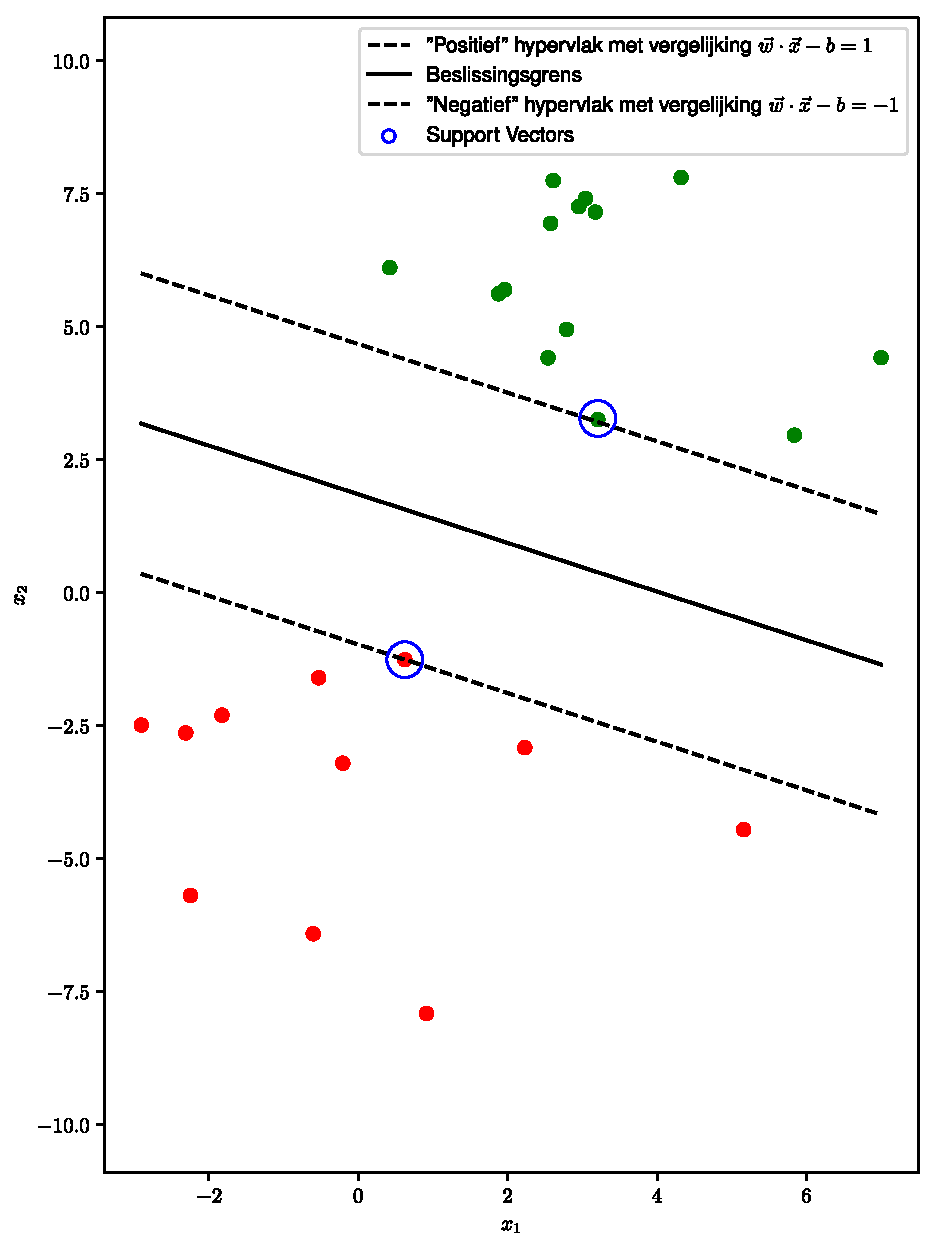
\includegraphics[width=.7\textwidth]{svm}
	\caption{Twee lineair scheidbare wolken van punten. De kleuren van de punten duiden aan tot welke klasse ze behoren.}
	\label{fig:svm}
\end{figure}

De marge is het gebied tussen deze twee hypervlakken. De breedte van hiervan is gelijk aan \(\frac{2}{\norm{\vec{w}}}\) en aangezien we die breedte willen maximaliseren, zullen we m.a.w. dus \(\norm{\vec{w}}\) trachten te minimaliseren.

\subsection{Trainen van het model}

Als de dataset twee lineair scheidbare 'wolken' vormt en er geen \textit{outliers} - punten die niet tot de juiste wolk behoren - zijn, is het bepalen van de maximale marge vrij makkelijk. Het wordt moeilijker wanneer er wel \textit{outliers} zijn en de twee wolken dus niet meer perfect lineair scheidbaar zijn, zonder dat punten aan de verkeerde kant van de twee hyperplanes belanden.

Daarom voeren we nu de \textit{hinge loss} in. Dit is een soort foutterm die we toevoegen aan punten die niet goed of met geen grote zekerheid worden geclassificeerd. Deze \textit{hinge loss} wordt berekend door de formule \[\max{(0,1-y_i(\vec{w}\cdot\vec{x}_i-b))}\]. Deze foutterm laat ons toe om de fouten te beperken, terwijl we de marge maximaliseren. Voor elk punt hebben we dan twee mogelijkheden wat de waarde van de \textit{hinge loss} betreft:

\begin{enumerate}
	\item Het punt met afhankelijke variabele \(y_i\) werd correct geclassificeerd.
	
	Dan ligt het punt dus aan de juiste kant van een van de twee hyperplanes. In dit geval is \(y_i(\vec{w}\cdot\vec{x}_i-b)\ge1\) en zal \(1 - y_i(\vec{w}\cdot\vec{x}_i-b)\le0\). Omdat de \textit{hinge loss} het maximum neemt van 0 en dit laatste getal - dat ofwel ook 0, ofwel negatief is - zal de \textit{hinge loss} in dit geval 0 zijn.
	
	\item Het punt ligt in de marge of het punt ligt aan de verkeerde kant van de belissingslijn. 
	
	De \textit{hinge loss} wordt dan \(1 - y_i(\vec{w}\cdot\vec{x}_i - b)\). Indien het datapunt binnen de marge ligt, zal de hinge loss tussen 0 en 1 liggen. Het punt wordt dan met lagere zekerheid geclassificeerd, maar we willen het ook niet te hard bestraffen. Indien een datapunt buiten de marge, maar aan de verkeerde kant van de beslissingslijn ligt, zal de \textit{hinge loss} groter dan 1 zijn. We willen het model wel hard bestraffen, want zo'n fouten willen we miniem houden.
\end{enumerate}

Om het SVM-model te trainen, moeten we nu dus met twee zaken rekening houden. Enerzijds willen we \(\norm{\vec{w}}\) minimaliseren om een zo groot mogelijke marge te bekomen anderzijds willen we de \textit{hinge loss} of strafterm zo klein mogelijk houden. We voeren een kostfunctie \(J\) in en zoeken het minimum \(\min_{w, b}J\) van deze functie. Het minimalisatieprobleem wordt dan gegeven door de formule \[\min_{w, b}J=\min_{w, b}\left[\frac{1}{n}\sum_{i=1}^n{\max{[0,1-y_i(\vec{w}\cdot\vec{x}_i-b)]}} + \lambda\cdot{||\vec{w}||}^2\right]\].

Hierbij is \(\frac{1}{n}\sum_{i=1}^n{\max{[0,1-y_i(\vec{w}\cdot\vec{x}_i-b)]}}\) de gemiddelde \textit{hinge loss}, dus de gemiddelde foutterm die werd toegekend over alle \(n\) datapunten in de dataset. De tweede term \(\lambda\cdot{||\vec{w}||}^2\) regelt het evenwicht tussen enerzijds het minimaliseren van de fouten op de trainingsdata en anderzijds het maximaliseren van de marge. \(\lambda\) is een metaparameter van het model en deze parameter vertelt aan het model hoeveel belang we hechten aan het minimaliseren van \(\norm{\vec{w}}\). 

Als \(\lambda\) klein - en eventueel zelfs \(0\) - is, komt het berekenen van een minimale kostfunctie $J$ neer op het op nul zetten van zo veel mogelijke \textit{hinge losses} van zo veel mogelijk punten. Dit resulteert in een kleine marge. Als \(\lambda\) groot is, ligt er meer nadruk op het minimaliseren van de grootte van \(\norm{\vec{w}}\) en dan spelen de \textit{hinge losses} een minder grote rol. Hoe kleiner \(\norm{\vec{w}}\), hoe groter de marge, want de marge is \(\frac{2}{\norm{\vec{w}}}\) breed. We concluderen dat \(\lambda\) resulteert in een grotere marge, zoals te zien is in figuur \ref{fig:lambda}.

\begin{figure}
	\centering
	\includegraphics[width=\textwidth]{lambda}
	\caption{De invloed van de metaparameter \(\lambda\)op het SVM-model. Een grote \(\lambda\) resulteert in een grote marge, een kleine \(\lambda\) resulteert in een kleine marge.}
	\label{fig:lambda}
\end{figure}

%Beschouw nu opnieuw de twee situaties die we eerder besproken hebben: in situatie 1 werd een punt correct geclassificeerd, in situatie 2 lag een punt in de marge of werd het verkeerd geclassificeerd. De kostfunctie \(J_i\) voor een enkel datapunt in geval 1 is dan \(\lambda\cdot{\norm{\vec{w}}}^2\). Dus geldt \(\frac{d}{dw}(J_i)=2\lambda w\) en \(\frac{d}{db}(J_i)=0\). De kostfunctie \(J_i\) voor een enkel datapunt in geval 2 is \(1-y_i(\vec{w}\cdot\vec{x}_i-b) + \lambda\cdot{||\vec{w}||}^2\). Dus geldt \(\frac{d}{dw}(J_i)=2\lambda w-y_i\cdot x_i\) en \(\frac{d}{db}(J_i)=y_i\).
	
\end{document}